% !Mode:: "TeX:UTF-8"

\documentclass[literaturereview]{zjutreport}
\graphicspath{{figures/}}  % 定义所有的eps文件在 figures 子目录下

\begin{document}           % 开始全文

%论文题目:{中文}
\zjuttitle{基于内存数据库的大数据应用系统的设计与实现}
%作者:{中文姓名}{学号}
\zjutauthor{陈佳鹏}{200926630503}
%指导教师:{导师中文名}
\zjutmentor{陈~~~~波}
%个人信息:{毕业年份}{专业名称}
\zjutinfo{2013}{软件工程}
%学院信息:{学院中文}
\zjutcollege{计算机科学与技术学院}
%日期:{提交日期}
\zjutdate{2013年03月}

% !Mode:: "TeX:UTF-8"
%%============================================================
%% 中文封面
\thispagestyle{empty}
\pdfbookmark[-1]{\zjuttitlec}{zjutreportcover}
\phantomsection \label{zjutreportcover}
\vspace*{-2.5mm}
% 校名
\begin{center}
   
\includegraphics[width=98.40mm]{figures/zjut}
\end{center}
\vspace*{9.66mm}
\centerline{\songti\yihao{\reporttitle}}
\vspace*{10.0mm}
\centerline{\heiti\xiaoer\textbf{(\zjutgrade\ 届)}}
\vspace*{8.5mm}
% 校徽
\begin{center}
  
\includegraphics[width=27.3mm]{figures/zjutlogo}
\end{center}

\vspace*{0.0mm}
\renewcommand{\arraystretch}{1.0}
\hspace*{7.4mm}
{\songti\erhao{论文题目}}
\hspace{6mm}
\begin{minipage}[t]{95mm}
    \linespread{1.1}{\songti\xiaoer\uline{\zjuttitlec}}
\end{minipage}
\vspace*{9mm}
\begin{center}
    \setlength{\arrayrulewidth}{0.5pt}
    {\songti\sihao
        \renewcommand{\arraystretch}{1.4}
        \begin{tabular}{lc}
            作者姓名 \qquad &  \zjutauthornamec \\ \cline{2-2}
            指导教师\qquad &  \zjutmentorc\\ \cline{2-2}
            \\
            学科(专业)\qquad &  \zjutmajor \\ \cline{2-2}
            所在学院\qquad &  \zjutcollegec \\ \cline{2-2}\cline{2-2}
            提交日期\qquad & \zjutsubmitteddatee \\ \cline{2-2}
        \end{tabular}
    }
\end{center}

      % 封面

\frontmatter

\pagenumbering{Roman}
\begingroup % 在组内的chapter不换行
\let\clearpage\relax % chapter之后不换页

%%%%%%%%%% 标题 %%%%%%%%%%
\titleformat{\chapter}[block]{\sihao\heiti\filcenter\bfseries}{\CJKnumber{\thechapter}}{1ex}{}{} % 标题居中,黑体三号
\chapter*{基于内存数据库的大数据应用系统的设计与实现}
\titleformat{\chapter}[block]{\xiaosi\heiti}{\CJKnumber{\thechapter}、}{1ex}{}{} % 恢复标题居左,黑体四号

%%%%%%%%%% 摘要 %%%%%%%%%%
% !Mode:: "TeX:UTF-8"

%%%%% 摘要 %%%%%
\abstractc{本文是基于内存数据库的大数据应用系统的设计与实现的一篇文献综述,先介绍项目的由来及其研究意思,然后介绍项目的国内外研究现状及难点以定位项目开发的一个大环境,明确当前同类项目的研究情况。接着本文简述内存数据库系统的结构,紧接着介绍系统开发中所需的关键技术。}

%%%%% 关键词 %%%%%
\keywordsc{内存数据库,索引结构,并发控制,T树,数据恢复,影子内存,混合日志}
     % 中文摘要

%%%%%%%%%% 正文 %%%%%%%%%%
\mainmatter
% \makeatletter
\chapter{引言}
1969年,埃德加•弗兰克•科德(Edgar Frank Codd)发表了一篇划时代的论文,首次提出了关系数据模型的概念。但可惜的是,刊登论文的“IBM Research Report”只是IBM公司的内部刊物,因此论文反响平平。1970年,他再次在刊物《Communication of the ACM》上发表了题为“A Relational Model of Data for Large Shared Data banks”(大型共享数据库的关系模型)的论文,终于引起了大家的关注。

科德所提出的关系数据模型的概念成为了现今关系型数据库的基础。当时的关系型数据库由于硬件性能低劣、处理速度过慢而迟迟没有得到实际应用。但之后随着硬件性能的提升,加之使用简单、性能优越等优点,关系型数据库得到了广泛的应用。

但是现如今随着互联网的不断发展,各种类型的应用层出不穷,所以导致在这个云计算的时代,对技术提出了更多的需求,传统关系型数据库面临很多问题,主要体现在下面这四个方面:

1. 低延迟的读写速度:应用快速地反应能极大地提升用户的满意度;

2. 支撑海量的数据和流量:对于搜索这样大型应用而言,需要利用PB级别的数据和能应对百万级的流量;

3. 大规模集群的管理:系统管理员希望分布式应用能更简单的部署和管理;

4. 庞大运营成本的考量:IT经理们希望在硬件成本、软件成本和人力成本能够有大幅度地降低;

虽然关系型数据库已经在业界的数据存储方面占据不可动摇的地位,但是由于其天生的几个限制,使其很难满足上面这几个需求:

1. 扩展困难:当需要表与表之间Join操作的时候,数据库就不能很好的进行扩展;

2. 读写速度慢:当数据量达到较大规模的时候,很容易发生死锁的问题,直接导致读写速度急剧下降的问题。

3. 成本高:企业级数据库的License价格很惊人,并且随着系统的规模,而不断上升;

4. 有限的支撑容量:现有关系型解决方案还无法支撑Google这样海量的数据存储;

这就促使了内存数据库(Main Memory Database,MMDB)的诞生。MMDB完全抛弃了传统数据库
对数据的管理方式,将数据完全放在内存中。此外,MMDB对缓存,索引,高并发操作等在这些方面
上也做了相当大的改进,这样一来,MMDB对数据的处理速度相对于磁盘数据库能快几倍甚至十几倍。MMDB
的目标,也是其最大的优势,就是利用内存来提高吞吐量和降低延迟,现在一些对响应时间要求较高
的程序,比如金融交易,电信等系统,都会使用MMDB。

\chapter{与传统数据库的异同}
磁盘数据库:将数据以物理文件的形式组织在硬盘上,是目前商业上应用最多,发展时间长,比较成熟的数据库。当读取数据时,数据块需要从磁盘中加载(也可说是复制或拷贝)到内存中。如果需要更新数据时,方式是先修改该部分数据在内存中的缓存,也就是副本,之后以同步或者异步的方式将修改完的数据重新写回硬盘。这样一来,会产生大量I/O操作,对性能有着很大影响。但是,这样也有好处,如果数据量很大的话(T级,P级),就可以储存在硬盘中。

内存数据库:将数据完全储存在内存,硬盘只是用于备份的数据库,是一种目前商业上应用不多,发展时间较短,还未成熟的数据库。目前也主要用于金融交易,电信等一些响应要求和性能要求较高的系统。把数据全都放在内存中的明显好处就是不需要做磁盘I/O,这样性能上相比于传统的磁盘数据库有着大步的飞跃。由于数据都放在内存中,内存数据库必须对数据的组织读取等做了一定的优化。但是,虽然现在已经出现了接近T级别的内存,但是由于内存大小的限制,内存数据库所能承受的数据量相比于传统磁盘数据库还是小很多。所以,现在流行的架构是两者同时使用,一些”热“数据储存在内存数据库中以便快速响应,后端磁盘数据库通过异步操作进行存储工作。

内存数据库和磁盘数据库一样,都是数据库产品,它们都有事务,都遵循ACID原则,允许并发访问并有锁机制。此外,为了保证数据的稳定性和安全性,它们也都有备份和恢复机制。内存数据库和磁盘数据库一样,都提供JDBC等用于开发的API及连接组件。

\chapter{主流内存数据库}
\section{Oracle TimesTen}
Oracle TimesTen内存数据库是一个功能全面的关系型内存数据库,旨在通过在应用层的运行,加速处理响应时间和关键任务型应用所需的高吞吐量。从某种角度上来看,TimesTen也是一种Cache机制,是磁盘数据库的‘Cache’,通过物理内存中的数据存储区的直接操作,减少了到磁盘间的I/O交互。TimesTen中的这个Ten据说就是指速度能达到基于磁盘的RDBMS10倍。

\section{IBM SolidDB}
IBM solidDB是一个关系内存型数据库软件,可以以极高的速度交付数据,执行速率高达传统数据库的10倍。它使用熟悉的SQL语言,使应用程序能够达到每秒数万个事务的吞吐量,其响应时间需要用毫秒来度量,为应用程序提供了具有亚秒级故障转移速率的极高的数据可用性。无论是部署为IBM-DB2或IDS的缓存,还是部署为独立的数据库,solidDB都能够以极快的速率交付性能关键型数据。

\section{eXtremeDB}
eXtremeDB是美国麦科捷科技有限公司(McObject LLC)开发的一款专业的嵌入式实时内存数据库,它具有高性能,低开销,稳定可靠的极速实时数据管理能力,广泛应用在嵌入式数据管理领域及服务器实时数据管理领域。
eXtremeDB完全工作在主内存中,不基于文件系统,减少了诸如磁盘访问、文件I/O操作、缓存同步等开销,使得eXtremeDB的存取速度提高到极限;通过数据库定义语言面向应用系统定制的API使得eXtremeDB能够面向应用最优化;事件触发、字段优先级等特色使得eXtremeDB管理实时数据时具有确定性。

eXtremeDB根据用户需求定义的API使得eXtremeDB与应用程序无缝集成。因此,eXtremeDB不仅在系统中嵌入,而且“嵌入”在应用程序中,是一种真正的嵌入式实时数据库。在资源紧凑的系统中,eXtremeDB基本内存开销在60K到100K左右;对于大量实时数据需管理的情形,eXtremeDB最大一表格的记录总数可以达到2,147,483,647条。

\section{SAP HANA}
SAP HANA是一款面向数据源的、灵活、多用途的内存应用设备,整合了基于硬件优化的SAP软件模块,通过SAP主要硬件合作伙伴提供给客户。SAP HANA提供灵活、节约、高效、实时的方法管理海量数据。利用HANA,企业可以不必运行多个数据仓库、运营和分析系统,从而削减相关的硬件和维护成本。SAPHANA将在内存技术基础上,为新的创新应用程序奠定技术基础,支持更高效的业务应用程序,如:计划、预测、运营绩效和模拟解决方案。

\chapter{系统实现技术方法研究}
\section{数据的组织结构}
由于内存数据库对性能要求十分高,所以大量使用了内存的共享机制。此外,指针也广泛的应用于内存数据库中,由于其长度固定的特性,指针可以很好的处理变长字段的问题。通常而言,内存数据库一般采用分级结构来储存数据,分级一般包括“段”和“分区”,两者明显的区别在于段是变长的,分区是固长的,段由若干个分区组成。

拿IBM的Starburst作为例子来说,分区是最基本的单元,主要任务是内存的分配和回收工作。图~\ref{fig:starburst}~描述了
Starburst的内存数据组织结构图。

\begin{figure}[htbp]
\centering
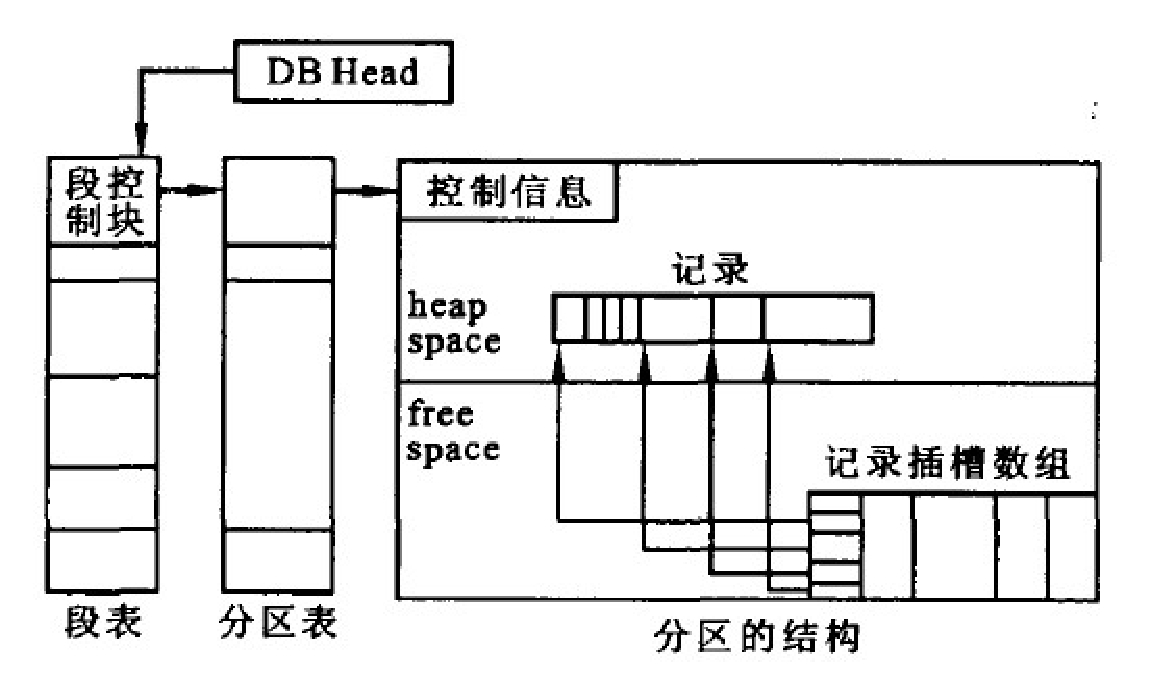
\includegraphics[width=0.4\textwidth]{starburst}
\caption{Starburst内部结构}\label{fig:starburst}
\vspace{\baselineskip}
\end{figure}

从图~\ref{fig:starburst}~中可以看到:记录插槽中包含了一个指针,这个指针指向了每条记录的的地址,所以记录存在Heap区,通过Free区记录插槽可以对记录进行读取。上文说过,由于指针长度不变性,它可以很好的用来解决表示不等长字段的问题。当程序要访问一个记录时,可以根据其所在的段号、分区号、以及偏移量在快速确定到此条记录。

\section{数据索引}
\subsection{T树}
文献[16]主要介绍了T树以及其在内存数据库中的使用情况,并与B树做了一定的比较:
磁盘数据库采用的索引结构主要是B/B$+$树,其设计目标是减少访问磁盘数据的IO次
数。而在MMDB中,通常采用了一种新的索引结构T树,其设计目标是减少内存开
销和CPU指令数。T树是由AVL树和B树发展而来,是一颗特殊平衡的二叉树(AVL),
它的每个节点存储了按键值排序的一组关键字。T树除了较高的节点空间占有率,
遍历一棵树的查找算法在复杂程度和执行时间上也占有优势。现在T树己经成为内
存数据库中最主要的一种索引方式。T树的结点如图~\ref{fig:treenode}~所示。

\begin{figure}[htbp]
%%% TODO 插入T树node图  from 内存数据库关键技术研究.pdf%%%
\centering
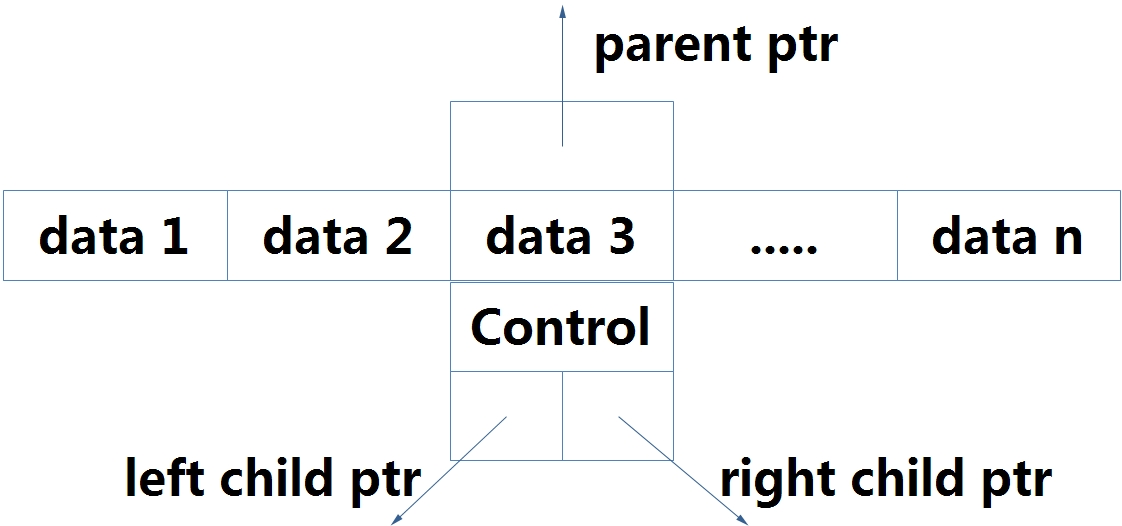
\includegraphics[width=0.4\textwidth]{treenode}
\caption{T树节点}\label{fig:treenode}
\vspace{\baselineskip}
\end{figure}

T树保持了AVL树二分查找高效率的同时也像B树一样,每个节点的充满程度
保持在半满和全满之间,这样索引一般不再需要溢出块,由插入和删除所引起的数据移动通常只需在一个节点内
进行,减少了树的旋转操作,因此T树保持了B树
优异的更新和存储特性。由于索引和数据全在内存中,T树节点中不需
要存放N个索引键值指针对,只需存放指向内存中相应记录对应
字段的指针即可,这样一来索引中变长字段的存储不再是问题,同时也节省了大量的空间。

\subsection{Hash}
文献[19]大致介绍了Hash在内存数据库中的使用情况,Hash的作用就是为了快速地定位数据库的记录,MMDB中广泛使用的哈希索引有以下几种:
链接桶哈希(Chained Bucket hashing)、可扩展哈希(extendible hashing)、
线性哈希(linear hashing)、修正的线性哈希(modified linear hashing)
等。其中链接桶的哈希使用静态结构处理冲突,速度很快,但不适合动态环境。
虽然使用Hash能够快速地访问数据库,且易于实现,但不能满足一定
范围的检索需求。

\section{并发控制}
文献[16]中引用IBM的Starburst系统作为例子,阐述了如何使用封锁的机制来保证事务的ACID特性:
把锁分成两种级别,记录级锁、表级锁。两中锁在开销方面明显是表级锁要小于记录级锁。所以,一般情况下推荐使用表级锁,但是当发生多个事务在访问表并被其他事务阻塞时,应该用记录级别锁代替表级锁。

由于事务所需的数据完全在内存中,事务能高效的执行,但封锁产生的代价会严重影响到总体的性能,因此可采用如下的方法来减少这个代价:

1)采用较大的锁粒度(如表级锁),因为数据常驻内存后,对数据的竞争已
很低,细粒度锁的优点对改善性能的意义已不大

2)采用乐观加锁方式

3)减少锁的类型

4)将锁信息存储在数据本身

\section{恢复机制}
内存数据库的恢复机制与磁盘数据库的恢复机制没有本
质上的区别。除了使用稳定内存的恢复机制之外,其他恢复
机制都需要将数据写到磁盘上,这在很大程度上影响了内存
数据库的性能,这是需要研究解决的关键技术。

对于将日志写在何处以及何时将日志写人磁盘的
问题,一些研究者提出了预提交、组提交等方法来降低日志I/O的代价,并
且提出使用稳定内存存储日志的方法:首先将日志存储在稳定内存中,然后
提交事务,再异步地把日志写入磁盘。在内存数据库中,只有在事务提交写日志、
执行Checkpoint、以及系统故障恢复时才需要访问磁盘,基于以上分析,重
新设计MMDB的事务提交策略和Checkpoint方式,对改善系统性能至关重要。


\subsection{事务提交}
为保证事务的ACID特性,事务提交时必须强制写日志到磁盘,因此写日志成为
系统的瓶颈。如何提高MMDB中事务提交的速度,常用以下方法:

1)使用稳定内存

2)组提交

3)只记录ReDo日志

\chapter{总结}
内存数据库是一个较新的研究领域.由于它具有传统的磁盘数据库无法比拟
的优越性,已经引起了数据库领域的广泛关注与此同时.它也提出了很多需
要研究和探讨的新课题.必须研究设计与之相适应的数据结构和算法、相应
的各种管理技术.才能最大限度地发挥驻留内存的优越性。相信在不久的将
来.随着硬件、软件技术的不断发展.内存数据库将有非常广泛的应用。
在下一代网络中,随着业务智能的提高,数据处理的复杂度、规模和性能要
求越来越高,采用MMDB或内存数据管理中间件产品来改善系统性能将不可避
免。

% \makeatother
\backmatter
\endgroup % 组结束
%%%%%%%%%% 参考文献 %%%%%%%%%%
\clearpage % 显式换页,使书签定位准确
\bibliographystyle{unsrt}
\bibliography{references/reference}
\nocite{*}                                   % 若将此命令屏蔽掉,则未引用的文献不会出现在文后的参考文献中。

%%%%%%%%%% 附录 %%%%%%%%%%
%\appendix
%% !Mode:: "TeX:UTF-8"
%
% XXX refactor 暂时当静态页面处理
% 
\chapter{附录}

\phantomsection

\addcontentsline{toc}{section}{附录1 毕业设计文献综述}
\addcontentsline{toc}{section}{附录2 毕业设计开题报告}
\addcontentsline{toc}{section}{附录3 毕业设计外文翻译}
\hspace*{7.0mm}
\hspace*{4.0mm}
\begin{minipage}[t]{95mm}
    \heiti\bfseries{
    \sectionmark{附录1 毕业设计文献综述}
    附录1 毕业设计文献综述

    \vspace*{7.0mm}

    \sectionmark{附录2 毕业设计开题报告}
    附录2 毕业设计开题报告

    \vspace*{7.0mm}

    \sectionmark{附录3 毕业设计外文翻译}
    附录3 毕业设计外文翻译}
\end{minipage}


            % 附录

\end{document}                                  % 结束全文
